\section{Einsatzbereich}

\begin{tcolorbox}
    \textbf{Sequenzdiagramme} stellen Verhalten auf der Ebene einer Interaktion dar.
\end{tcolorbox}

\noindent
Bei Sequenzdiagrammen werden i.d.R. Schnittstellen zwischen \textbf{Kommunikationspartnern} modelliert.\\

\noindent
Das \textbf{Modellierungskonzept}\footnote{
s. Abschnitt~\ref{sec:sprachaufbau-der-uml-2.0}
} \textit{Interaktion} gibt einer Reihe von Diagrammen einen gemeinsamen Namen; die \textit{Interaktion} gibt dem Sequenzdiagramm hierbei einen funktionalen Rahmen, der auch modelliert wird (s. Abbildung~\ref{fig:interaktionsrahmen}).\\

\begin{figure}
    \centering
    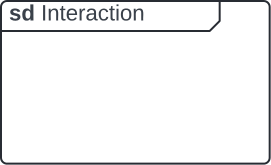
\includegraphics[scale=0.5]{part three/Sequenzdiagramme/img/interaktionsrahmen}
    \caption{Interaktionsrahmen. \textbf{sd} steht für \textit{Sequence Diagram} (Quelle: in Anlehnung an \cite[596]{UML17})}
    \label{fig:interaktionsrahmen}
\end{figure}

\noindent
Interaktionsrahmen können Attribute verhalten, die während der Interaktion gesetzt und gelesen werden können.\\

\noindent
Also Voraussetzung für das Beschreiben von Verhalten ist der Entwurf der beteiligten Kommunikationspartner gegeben, was i.d.R. durch das \textbf{Klassendiagramm} geschieht.\\
In demm Fall sind die Kommunikationspartner dann \textit{Objekte}.\\

\noindent
Interaktionen könenn aber auch auf Ebene von Systemkomponenten definiert werden, um Systemverhalten zu modellieren\footnote{
Kommunikationspartner kann dann bspw. ``Datenbankmanagementsystem`` sein.
}.\\

\noindent
In der \textbf{Analysephase} können Sequenzdiagramme eingesetzt werden, um die Kommunikation der bis dahin ausgemachten \textbf{Geschäftsobjekte} zu modellieren, oder um \textbf{Anwendungsfälle} weiter zu spezifizieren.